\documentclass[11pt,a4paper]{article}
\usepackage[utf8]{inputenc}
\usepackage[T1]{fontenc}
\IfFileExists{french.ldf}{\usepackage[french]{babel}}{\usepackage[english]{babel}}
\usepackage{amsmath,amssymb,amsthm}
\usepackage{geometry}\geometry{margin=2.4cm}
\usepackage{listings}
\usepackage{xcolor}
\usepackage{enumitem}
\usepackage{fancyhdr}
\usepackage{lmodern}
\usepackage{titlesec}
\usepackage{tikz}
\usetikzlibrary{arrows.meta,positioning,calc}
\usepackage{hyperref}
\hypersetup{colorlinks=true, urlcolor=[RGB]{2,101,115}, linkcolor=black, citecolor=black}

\definecolor{cnc}{RGB}{2,101,115}
\definecolor{codebg}{RGB}{247,249,251}
\definecolor{cmt}{RGB}{110,120,130}

\lstdefinestyle{pseudo}{
  mathescape=true, basicstyle=\ttfamily\small, backgroundcolor=\color{codebg},
  keywordstyle=\bfseries, commentstyle=\color{cmt}\itshape,
  morekeywords={Entree,Sortie,pour,tant,que,si,alors,sinon,renvoyer,faire,fin,retourner,
    Fonction,Algorithme,de,a,dans,chaque,vide,empiler,depiler,Donnees,Resultat},
  numbers=left, numberstyle=\tiny\color{cmt}, numbersep=8pt,
  frame=single, rulecolor=\color{gray!40}, columns=fullflexible, showstringspaces=false,
  breaklines=true, extendedchars=true, inputencoding=utf8,
  literate={é}{{\'e}}1 {è}{{\`e}}1 {à}{{\`a}}1 {ê}{{\^e}}1 {î}{{\^i}}1 {ç}{{\c c}}1
           {ù}{{\`u}}1 {ô}{{\^o}}1 {û}{{\^u}}1 {'}{{'}}1
}
\lstset{style=pseudo}

\AtBeginDocument{\renewcommand{\proofname}{\bfseries Démonstration}}
\theoremstyle{plain}
\newtheorem{theoreme}{Théorème}
\newtheorem{lemme}[theoreme]{Lemme}
\newtheorem{proposition}[theoreme]{Proposition}
\newtheorem{corollaire}[theoreme]{Corollaire}
\theoremstyle{definition}
\newtheorem{defi}[theoreme]{Définition}
\newtheorem{remarque}[theoreme]{Remarque}
\newtheorem{exemple}[theoreme]{Exemple}

\pagestyle{fancy}\fancyhf{}
\lhead{\small Épreuve de modélisation --- Informatique}
\rhead{\small Consensus réparti : le protocole Casper}
\cfoot{\thepage}
\renewcommand{\headrulewidth}{0.4pt}
\titleformat*{\section}{\large\bfseries\scshape\color{cnc}}
\titleformat*{\subsection}{\bfseries\color{cnc}}

\newcommand{\Cc}{\mathcal{C}}
\newcommand{\Vv}{\mathcal{V}}
\newcommand{\Ll}{\mathcal{L}}
\newcommand{\Jj}{\mathcal{J}}
\newcommand{\Ff}{\mathcal{F}}
\newcommand{\Fa}{\mathrm{Faut}}
\newcommand{\anc}{\preccurlyeq}
\newcommand{\ancs}{\prec}

\begin{document}
\thispagestyle{fancy}

\begin{center}
{\small\scshape Agrégation --- Épreuve orale de modélisation}\\[2pt]
{\small\scshape Option informatique}\\[10pt]
\rule{0.92\linewidth}{0.5pt}\\[8pt]
{\LARGE\bfseries Finalité et responsabilité}\\[4pt]
{\LARGE\bfseries dans un consensus réparti}\\[8pt]
{\large\itshape Le protocole Casper}\\[10pt]
\rule{0.92\linewidth}{0.5pt}\\[10pt]
{\small Texte rédigé d'après V.~Buterin et V.~Griffith, \emph{Casper the Friendly Finality
Gadget},\\ Ethereum Foundation, arXiv:1710.09437v4, 2019.}\\[8pt]
{\small \href{https://orcid.org/0000-0002-6108-7176}{\textbf{Pr Agrégé El Hadiq Zouhair}}
\quad---\quad \href{https://cpgeacademy.org}{\textbf{cpgeacademy.org}}}
\end{center}

\vspace{4mm}
\noindent\fcolorbox{gray}{gray!5}{\begin{minipage}{0.975\linewidth}\small
\textbf{Recommandations du jury.} Il est rappelé que le jury n'exige pas une compréhension
exhaustive du texte. Vous êtes laissé(e) libre d'organiser votre discussion comme vous
l'entendez. Des suggestions de développement, largement indépendantes les unes des autres,
vous sont proposées en fin de texte. Vous n'êtes pas tenu(e) de les suivre. Il vous est
conseillé de mettre en lumière vos connaissances à partir du fil conducteur constitué par le
texte. Le jury appréciera que la discussion soit accompagnée d'exemples traités sur
ordinateur.
\end{minipage}}
\vspace{3mm}

%=====================================================================
\section{Le problème}
%=====================================================================

Un \emph{registre réparti} est une base de données répliquée sur un grand nombre de machines
qui ne se font pas confiance, connectées par un réseau non fiable, et dont une fraction
inconnue peut se comporter de manière arbitrairement malveillante (modèle
\emph{byzantin}). Le problème central est celui du \textbf{consensus}~: faire converger tous
les participants honnêtes vers une même suite de transactions.

Les systèmes de type \emph{preuve de travail} (Bitcoin) résolvent ce problème de façon
probabiliste~: un bloc n'est jamais définitivement acquis, il devient seulement de plus en
plus improbable qu'il soit révisé. À l'opposé, les algorithmes issus de la tradition BFT
(\textsc{pbft}, Tendermint) offrent une \textbf{finalité} déterministe~: un bloc validé ne
peut plus être révisé, sous l'hypothèse que moins d'un tiers des participants sont
byzantins.

Transposer ces algorithmes au cadre de la \emph{preuve d'enjeu}, où l'influence d'un
participant est proportionnelle au capital qu'il immobilise, se heurte au problème dit du
\emph{« rien en jeu »} (\emph{nothing at stake})~: voter simultanément pour deux branches
concurrentes ne coûte rien, alors qu'en preuve de travail cela exigerait de dédoubler sa
puissance de calcul. Le protocole \textbf{Casper} apporte une réponse à ce problème en
rendant la triche non seulement détectable mais \textbf{imputable}~: si deux blocs
incompatibles sont finalisés, on sait \emph{quels} participants ont fauté, et l'on peut
confisquer leur capital.

Ce texte propose une modélisation de Casper. On y formalise l'objet combinatoire sur lequel
le protocole opère (§\ref{sec:modele}), on démontre ses deux propriétés fondamentales
(§\ref{sec:surete}), on examine les questions algorithmiques que soulève sa mise en \oe uvre
(§\ref{sec:algo}), puis on discute deux extensions et leurs limites (§\ref{sec:limites}).

%=====================================================================
\section{Le modèle}\label{sec:modele}
%=====================================================================

\subsection{Arbre de blocs et points de contrôle}

Le mécanisme qui \emph{propose} les blocs (une chaîne à preuve de travail, dans la première
version de Casper) est extérieur au protocole~: Casper est une \emph{surcouche}. On le
modélise simplement par sa production.

\begin{defi}
Un \textbf{arbre de blocs} est un arbre enraciné fini $(\mathcal{B},g)$~; la racine $g$ est
le \emph{bloc génésis}, et le \emph{numéro} $\mathrm{nb}(b)$ d'un bloc est sa profondeur dans
$\mathcal{B}$.
\end{defi}

En régime normal, le mécanisme de proposition produit une simple liste chaînée~; mais la
latence du réseau ou une attaque délibérée engendrent inévitablement plusieurs fils d'un même
bloc. La tâche de Casper est de choisir, dans cet arbre, une unique chaîne canonique.

Raisonner sur l'arbre complet serait trop coûteux. On se restreint donc à un sous-arbre
espacé~:

\begin{defi}
Un bloc $b$ est un \textbf{point de contrôle} si $b=g$ ou si $\mathrm{nb}(b)\equiv 0
\pmod{100}$. Les points de contrôle, munis de la relation « plus proche ancêtre qui est un
point de contrôle », forment un arbre $\Cc$ enraciné en $r=g$, l'\textbf{arbre des points de
contrôle}. La \textbf{hauteur} $h(c)$ d'un point de contrôle est sa profondeur dans $\Cc$~;
ainsi $h(c)=\mathrm{nb}(c)/100$.
\end{defi}

On note $a\anc b$ (« $a$ est un ancêtre de $b$ ») la relation d'ordre partiel induite par
$\Cc$, et $a\ancs b$ sa version stricte. Deux points de contrôle $a$ et $b$ sont
\textbf{en conflit}, ce qu'on note $a\bowtie b$, lorsque ni $a\anc b$ ni $b\anc a$~: ils
appartiennent à deux branches distinctes.

\begin{remarque}
L'espacement de $100$ blocs est un compromis~: plus il est grand, plus le coût du protocole
est amorti, mais plus la finalisation est lente. C'est un paramètre de modélisation, non une
nécessité mathématique~; toute la théorie qui suit vaut pour un espacement quelconque.
\end{remarque}

\begin{center}
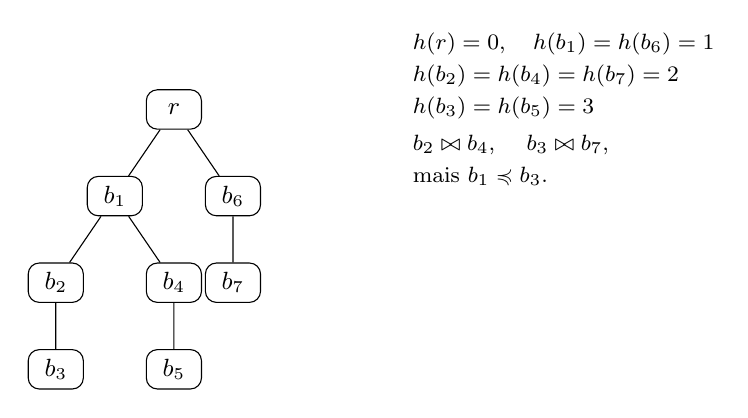
\begin{tikzpicture}[>=Stealth, every node/.style={draw, rounded corners, minimum width=7mm,
 minimum height=5mm, inner sep=2pt, font=\small}, level distance=11mm, sibling distance=15mm]
\node (r) {$r$}
  child {node {$b_1$}
    child {node {$b_2$} child {node {$b_3$}}}
    child {node {$b_4$} child {node {$b_5$}}}}
  child {node {$b_6$} child {node {$b_7$}}};
\node[draw=none, right=26mm of r, font=\footnotesize, align=left]
 {$h(r)=0,\quad h(b_1)=h(b_6)=1$\\[2pt]
  $h(b_2)=h(b_4)=h(b_7)=2$\\[2pt]
  $h(b_3)=h(b_5)=3$\\[4pt]
  $b_2\bowtie b_4$, \quad $b_3\bowtie b_7$,\\[2pt]
  mais $b_1\anc b_3$.};
\end{tikzpicture}

{\footnotesize\itshape Figure 1 --- Un arbre de points de contrôle. Chaque arête représente
$99$ blocs intermédiaires.}
\end{center}

\subsection{Validateurs, dépôts et votes}

\begin{defi}
Un \textbf{jeu de validateurs} est un ensemble fini $\Vv$ muni d'une application
$d:\Vv\to\mathbb{N}^{*}$, le \emph{dépôt}. On pose, pour $E\subseteq\Vv$,
$w(E)=\sum_{\nu\in E}d(\nu)$ et $T=w(\Vv)$. Une partie $E$ est une
\textbf{supermajorité} lorsque $w(E)\ge \tfrac{2}{3}T$.
\end{defi}

C'est ici le premier choix de modélisation notable~: la sécurité d'un système à preuve
d'enjeu ne dépend pas du \emph{nombre} de validateurs mais du \emph{capital} immobilisé. On
raisonne donc systématiquement avec la mesure $w$, et jamais avec le cardinal. Toutes les
fractions ($\tfrac23$, $\tfrac13$) s'entendent au sens de $w$.

\begin{defi}
Un \textbf{vote} est un quadruplet $\langle \nu, s, t, h(s), h(t)\rangle$ signé par $\nu$, où
$\nu\in\Vv$, et $s,t\in\Cc$. Il est \textbf{valide} lorsque $s\ancs t$. On dit que $s$ est la
\emph{source} et $t$ la \emph{cible}. Pour $(s,t)\in\Cc^2$, on note $E_{s\to t}$ l'ensemble
des validateurs ayant publié un vote valide de source $s$ et de cible $t$.
\end{defi}

Les hauteurs $h(s)$ et $h(t)$ sont redondantes avec $s$ et $t$~: elles figurent dans le
message pour que les conditions de la §\ref{sec:surete} soient vérifiables \emph{sans
connaître l'arbre}, donc localement et à moindre coût. C'est un point de modélisation
important~: les \emph{conditions de sanction} ne portent que sur les hauteurs, jamais sur la
topologie de l'arbre~; elles sont donc indépendantes de l'état de la chaîne.

\begin{defi}\label{def:noyau}
Un couple $(s,t)$ est un \textbf{lien de supermajorité}, noté $s\to t$, lorsque $E_{s\to t}$
est une supermajorité. On note $\Ll\subseteq\Cc^2$ l'ensemble des liens de supermajorité.

L'ensemble $\Jj$ des points de contrôle \textbf{justifiés} est la plus petite partie de $\Cc$
telle que
\[ r\in\Jj \qquad\text{et}\qquad \big(c\in\Jj \ \text{et}\ c\to c'\big)\Longrightarrow
c'\in\Jj . \]
Un point de contrôle $c$ est \textbf{finalisé} lorsque $c=r$, ou lorsque $c\in\Jj$ et qu'il
existe $c'$ fils direct de $c$ dans $\Cc$ tel que $c\to c'$. On note $\Ff$ l'ensemble des
points de contrôle finalisés.
\end{defi}

\begin{remarque}
La définition de $\Jj$ est celle d'un \emph{plus petit point fixe}~: l'opérateur
$\Phi(X)=\{r\}\cup\{c' : \exists c\in X,\ c\to c'\}$ est monotone sur le treillis complet
$(\mathcal{P}(\Cc),\subseteq)$, donc admet par le théorème de Knaster--Tarski un plus petit
point fixe, qui vaut $\bigcup_{k\ge 0}\Phi^k(\varnothing)$ puisque $\Cc$ est fini. On
reconnaît par ailleurs, en lisant $\Ll$ comme l'ensemble des arcs d'un graphe orienté sur
$\Cc$, que $\Jj$ est exactement l'ensemble des sommets \emph{accessibles depuis $r$}. Les
deux lectures — point fixe et accessibilité — conduisent à deux implantations différentes
(§\ref{sec:algo}).
\end{remarque}

\begin{exemple}
Sur la figure~1, supposons $\Vv=\{\alpha,\beta,\gamma,\delta\}$ de dépôts respectifs
$30,30,20,20$, donc $T=100$ et le seuil de supermajorité $\lceil 2T/3\rceil = 67$. Si
$\alpha,\beta,\gamma$ (de poids $80$) votent tous trois $r\to b_1$, $b_1\to b_2$ et
$b_2\to b_3$, alors $\Ll=\{(r,b_1),(b_1,b_2),(b_2,b_3)\}$, $\Jj=\{r,b_1,b_2,b_3\}$ et
$\Ff=\{r,b_1,b_2\}$~: le point $b_3$ est justifié mais pas encore finalisé.
\end{exemple}

Notons qu'un lien peut « sauter » des points de contrôle~: rien n'impose $h(t)=h(s)+1$ dans
la définition~\ref{def:noyau}. C'est précisément ce qui rend le protocole robuste à la perte
de messages, et c'est aussi ce qui rend les démonstrations qui suivent non triviales.

%=====================================================================
\section{Sûreté responsable et vivacité}\label{sec:surete}
%=====================================================================

\subsection{Les deux conditions de sanction}

\begin{defi}\label{def:comm}
Un validateur $\nu$ \textbf{faute} s'il publie deux votes distincts $\langle\nu,s_1,t_1
\rangle$ et $\langle\nu,s_2,t_2\rangle$ vérifiant l'une des deux conditions~:
\begin{itemize}[leftmargin=2.4em,itemsep=1pt]
\item[\textbf{(I)}] $h(t_1)=h(t_2)$~: \emph{deux votes distincts pour une même hauteur de
cible}~;
\item[\textbf{(II)}] $h(s_1)<h(s_2)<h(t_2)<h(t_1)$~: \emph{un vote strictement emboîté dans
un autre}.
\end{itemize}
On note $\mathrm{Faut}$ l'ensemble des validateurs fautifs. La preuve d'une faute étant un couple
de messages signés, elle peut être publiée dans la chaîne elle-même~; le protocole confisque
alors l'intégralité du dépôt du fautif.
\end{defi}

La condition (I) interdit de soutenir deux branches concurrentes à un même niveau. La
condition (II) est plus subtile~: elle interdit de « recouvrir » un vote par un autre, ce qui
reviendrait à revenir sur une décision déjà prise. Ces deux conditions sont \emph{locales}
(elles ne concernent qu'un validateur à la fois) et \emph{sans état} (elles ne portent que
sur les quatre hauteurs des deux messages).

\subsection{Le lemme d'intersection}

Tout repose sur l'observation élémentaire suivante.

\begin{lemme}[Intersection]\label{lem:inter}
Si $E_1$ et $E_2$ sont deux supermajorités, alors $w(E_1\cap E_2)\ \ge\ \dfrac{T}{3}$.
\end{lemme}

\begin{proof}
La mesure $w$ étant additive, $w(E_1\cup E_2)=w(E_1)+w(E_2)-w(E_1\cap E_2)$. Comme
$E_1\cup E_2\subseteq\Vv$ et que $w$ est croissante, $w(E_1\cup E_2)\le T$, d'où
$w(E_1\cap E_2)\ge \tfrac23 T+\tfrac23 T-T=\tfrac{T}{3}$.
\end{proof}

Ce lemme est le seul endroit où le seuil $\tfrac23$ intervient~; il explique pourquoi c'est
ce seuil, et pas un autre, qui est retenu. Le tiers ainsi dégagé est la « caution »~: c'est
lui qui sera détruit en cas d'attaque.

\begin{proposition}\label{prop:iiv}
Supposons $w(\mathrm{Faut})<T/3$. Alors~:
\begin{enumerate}[label=(\roman*),leftmargin=2.4em,itemsep=1pt]
\item si $s_1\to t_1$ et $s_2\to t_2$ sont deux liens distincts, alors $h(t_1)\ne h(t_2)$~;
\item si $s_1\to t_1$ et $s_2\to t_2$ sont deux liens distincts, l'inégalité
$h(s_1)<h(s_2)<h(t_2)<h(t_1)$ est impossible~;
\item pour toute hauteur $n$, il existe au plus un lien de supermajorité de hauteur de cible
$n$~;
\item pour toute hauteur $n$, il existe au plus un point de contrôle justifié de hauteur $n$.
\end{enumerate}
\end{proposition}

\begin{proof}
(i) Si $h(t_1)=h(t_2)$, le lemme~\ref{lem:inter} appliqué à $E_{s_1\to t_1}$ et
$E_{s_2\to t_2}$ donne $w(E_{s_1\to t_1}\cap E_{s_2\to t_2})\ge T/3$~; or tout validateur de
cette intersection a publié les deux votes distincts en cause, et faute donc par (I). D'où
$w(\mathrm{Faut})\ge T/3$, contradiction. (ii) est identique avec la condition (II). (iii) est une
reformulation de (i). (iv)~: pour $n=0$ seul $r$ convient~; pour $n\ge1$, deux justifiés
distincts de hauteur $n$ seraient les cibles de deux liens distincts de même hauteur de
cible, ce qu'exclut (iii).
\end{proof}

\subsection{Le théorème de sûreté responsable}

\begin{theoreme}[Sûreté responsable]\label{th:safety}
Si deux points de contrôle en conflit sont tous deux finalisés, alors
$w(\mathrm{Faut})\ \ge\ T/3$.
\end{theoreme}

Autrement dit~: une violation de la sûreté est impossible tant que moins d'un tiers du
capital triche, et, si elle survient, au moins un tiers du capital total est détruit — et l'on
sait à qui il appartenait.

\begin{proof}
Raisonnons par l'absurde en supposant $w(\mathrm{Faut})<T/3$, de sorte que la
proposition~\ref{prop:iiv} s'applique. Soient $a_m$ et $b_n$ deux points de contrôle
finalisés avec $a_m\bowtie b_n$, de fils directs $a_{m+1}$ et $b_{n+1}$ tels que
$a_m\to a_{m+1}$ et $b_n\to b_{n+1}$. Ces fils sont justifiés, puisque $a_m$ et $b_n$ le
sont.

\emph{Cas $h(a_m)=h(b_n)$.} Alors $a_m$ et $b_n$ sont deux justifiés distincts de même
hauteur, ce qui contredit (iv).

\emph{Cas $h(a_m)<h(b_n)$} (quitte à échanger les rôles). Comme $b_n\in\Jj$, la
définition~\ref{def:noyau} fournit une chaîne
\[ r=\beta_0\to\beta_1\to\dots\to\beta_k=b_n \]
de liens de supermajorité dont tous les termes sont justifiés~; les votes étant valides, on a
$\beta_i\ancs\beta_{i+1}$, donc $\big(h(\beta_i)\big)_i$ est strictement croissante et chaque
$\beta_i$ est un ancêtre de $b_n$.

\emph{Étape 1.} Aucune hauteur $h(\beta_i)$ ne vaut $h(a_m)$ ni $h(a_{m+1})$. En effet, si
$h(\beta_i)=h(a_m)$, alors (iv) donne $\beta_i=a_m$, donc $a_m\anc b_n$, ce qui contredit
$a_m\bowtie b_n$~; et si $h(\beta_i)=h(a_{m+1})$, alors $\beta_i=a_{m+1}$ et $a_m\anc
a_{m+1}\anc b_n$, même contradiction.

\emph{Étape 2.} On a $h(\beta_0)=0\le h(a_m)$ et $h(\beta_k)=h(b_n)>h(a_m)$, donc, l'étape 1
excluant les égalités, $h(b_n)>h(a_{m+1})$. L'ensemble $\{i : h(\beta_i)>h(a_{m+1})\}$ est
donc non vide~; soit $j$ son minimum. Alors $j\ge1$ et, par minimalité et par l'étape 1,
$h(\beta_{j-1})<h(a_m)$ (les valeurs $h(a_m)$ et $h(a_{m+1})=h(a_m)+1$ étant exclues).

\emph{Étape 3.} On dispose ainsi des deux liens de supermajorité $\beta_{j-1}\to\beta_j$ et
$a_m\to a_{m+1}$, avec
\[ h(\beta_{j-1})\ <\ h(a_m)\ <\ h(a_{m+1})\ <\ h(\beta_j), \]
configuration exclue par (ii). Contradiction.
\end{proof}

\begin{center}
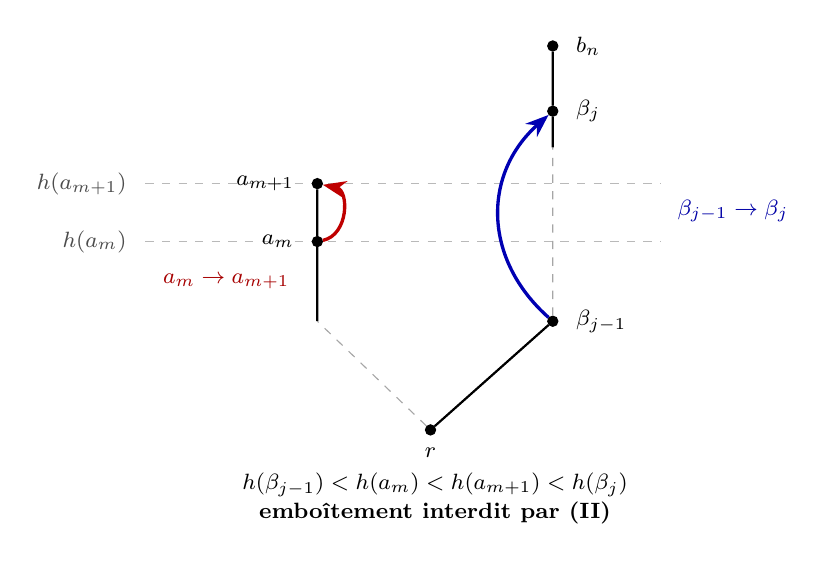
\begin{tikzpicture}[>=Stealth, xscale=1.15, yscale=0.92,
 pt/.style={draw, circle, inner sep=1.3pt, fill=black},
 lbl/.style={font=\footnotesize}]
% niveaux de hauteur
\foreach \y/\txt in {2.6/{$h(a_m)$}, 3.4/{$h(a_{m+1})$}} {
  \draw[dashed, gray!55] (-3.15,\y)--(2.55,\y);
  \node[lbl, gray!60!black, anchor=east] at (-3.25,\y) {\txt};
}
% branches
\node[pt] (r) at (0,0) {};
\node[lbl, below=1pt of r] {$r$};
\node[pt] (am)  at (-1.25,2.6) {};
\node[pt] (am1) at (-1.25,3.4) {};
\node[pt] (bp)  at (1.35,1.5) {};
\node[pt] (bj)  at (1.35,4.4) {};
\node[pt] (bn)  at (1.35,5.3) {};
\draw[gray!70, dashed] (r)--(-1.25,1.5);
\draw[thick] (-1.25,1.5)--(am)--(am1);
\draw[thick] (r)--(bp);
\draw[gray!70, dashed] (bp)--(1.35,3.9);
\draw[thick] (1.35,3.9)--(bj)--(bn);
% etiquettes des noeuds
\node[lbl, anchor=east] at (-1.4,2.6) {$a_m$};
\node[lbl, anchor=east] at (-1.4,3.4) {$a_{m+1}$};
\node[lbl, anchor=west] at (1.5,1.5) {$\beta_{j-1}$};
\node[lbl, anchor=west] at (1.5,4.4) {$\beta_j$};
\node[lbl, anchor=west] at (1.5,5.3) {$b_n$};
% liens de supermajorite
\draw[->, red!75!black, very thick, bend right=75] (am) to (am1);
\node[lbl, red!65!black, anchor=east] at (-1.45,2.05) {$a_m\to a_{m+1}$};
\draw[->, blue!70!black, very thick, bend left=42] (bp) to (bj);
\node[lbl, blue!65!black, anchor=west] at (2.62,3.02) {$\beta_{j-1}\to\beta_j$};
\node[lbl, align=center] at (0.05,-0.95)
  {$h(\beta_{j-1})<h(a_m)<h(a_{m+1})<h(\beta_j)$\\[1pt] \textbf{emboîtement interdit par (II)}};
\end{tikzpicture}

{\footnotesize\itshape Figure 2 --- Le c\oe ur de la preuve du théorème~\ref{th:safety}~: le
lien bleu enjambe strictement le lien rouge.}
\end{center}

\subsection{Vivacité plausible et règle de choix de fourche}

La sûreté seule est vide de sens~: un protocole qui ne finalise jamais rien est trivialement
sûr. Il faut lui adjoindre une garantie de progrès.

\begin{theoreme}[Vivacité plausible]\label{th:live}
Supposons qu'au moins $\tfrac23$ des validateurs suivent le protocole, et que ceux-ci ne
votent qu'avec une source justifiée. Alors, quel que soit l'historique des messages déjà
émis, il est toujours possible d'ajouter des liens de supermajorité finalisant un nouveau
point de contrôle, sans qu'aucun validateur ne faute.
\end{theoreme}

\begin{proof}
Soient $a$ le justifié de plus grande hauteur, et $b$ la cible de plus grande hauteur ayant
déjà fait l'objet d'un vote. Soit $a'$ un descendant de $a$ avec $h(a')=h(b)+1$ (il en existe
dès que le mécanisme de proposition continue à produire des blocs). Le vote $a\to a'$ ne
viole pas (I), car aucune cible de hauteur $h(b)+1$ n'a encore été votée~; il ne viole pas
(II) « par l'extérieur », car toute cible antérieure $t$ vérifie $h(t)\le h(b)<h(a')$, ni
« par l'intérieur », car toute source antérieure $s$ est justifiée donc vérifie $h(s)\le
h(a)$. On justifie ainsi $a'$~; on finalise ensuite $a'$ en ajoutant le lien $a'\to a''$ vers
un fils direct de $a'$, qui pour les mêmes raisons ne viole aucune condition.
\end{proof}

\begin{remarque}
L'hypothèse « les validateurs honnêtes ne votent qu'avec une source justifiée » est implicite
dans le texte original~; sans elle, un vote antérieur de source haute et de cible basse
pourrait se trouver emboîté dans le nouveau vote. Sa portée exacte, et la façon dont le
protocole l'impose, méritent discussion.
\end{remarque}

Le théorème~\ref{th:live} n'est pas seulement rassurant~: il \emph{dicte} la règle de choix
de branche, qui est ainsi \emph{correcte par construction}.

\begin{center}\fcolorbox{gray}{gray!5}{\begin{minipage}{0.88\linewidth}\centering\small
\textsc{Règle de choix de fourche.} \emph{Suivre la branche contenant le point de contrôle
justifié de plus grande hauteur.}
\end{minipage}}\end{center}

D'après (iv), ce point de contrôle est unique~; d'après le théorème~\ref{th:live}, c'est
au-dessus de lui, et de lui seul, qu'il est toujours possible de progresser. Un participant
qui suivrait la règle usuelle « la plus longue chaîne » pourrait au contraire se retrouver
sur une branche où plus rien ne peut être finalisé sans que quelqu'un sacrifie son dépôt.

%=====================================================================
\section{Aspects algorithmiques}\label{sec:algo}
%=====================================================================

\subsection{Calcul des justifiés et des finalisés}

L'arbre $\Cc$ est représenté par le tableau des pères, numéroté de sorte que le père d'un
n\oe ud porte toujours un numéro strictement plus petit — ce qui permet de calculer toutes
les hauteurs en un seul balayage, en $\Theta(n)$. Les relations $a\anc b$ et $a\bowtie b$ se
testent en remontant les liens de parenté, en $O(h(b))$~; le plus proche ancêtre commun
s'obtient en $O(h(a)+h(b))$ en égalisant d'abord les hauteurs.

Le calcul de $\Ll$ à partir d'une liste de $m$ votes est une simple agrégation par clé~:
\begin{lstlisting}
Algorithme LIENS($votes$, $d$, $T$)
  $P \leftarrow$ dictionnaire vide ; $U \leftarrow$ ensemble vide
  pour chaque vote $(\nu,s,t)$ de $votes$ faire
      si $(\nu,s,t) \notin U$ alors                # un validateur ne compte qu'une fois
          $U \leftarrow U \cup \{(\nu,s,t)\}$ ;  $P[(s,t)] \leftarrow P[(s,t)] + d(\nu)$
  renvoyer $\{\, (s,t) \;:\; 3\,P[(s,t)] \geq 2\,T \,\}$
\end{lstlisting}
soit $O(m)$ en moyenne. Le test $3w\ge 2T$ évite tout flottant~: les dépôts réels, exprimés
en \emph{wei} ($10^{18}$ par ether), dépassent largement la précision des flottants double
précision.

Le calcul de $\Jj$ suit la remarque faite après la définition~\ref{def:noyau}. Deux
implantations naturelles s'opposent~:
\begin{itemize}[leftmargin=1.4em,itemsep=2pt]
\item \emph{itération du point fixe}~: calculer $\Phi(\varnothing),\Phi^2(\varnothing),\dots$
jusqu'à stabilisation. Simple, directement calqué sur la définition, mais coûteux~: chaque
itération relit tout $\Ll$, d'où $O(|\Cc|\cdot|\Ll|)$ au pire~;
\item \emph{parcours de graphe}~: construire les listes d'adjacence de $(\Cc,\Ll)$ et
effectuer un parcours depuis $r$, en $O(|\Cc|+|\Ll|)$.
\end{itemize}
Le passage de l'une à l'autre est un exemple typique du gain obtenu en reconnaissant, derrière
une définition inductive, une structure de graphe. $\Ff$ s'en déduit en $O(|\Ll|)$~: il suffit
de parcourir les liens $(c,c')$ et de retenir $c$ lorsque $c\in\Jj$ et que $c'$ est le fils
direct de $c$.

\subsection{Détection des fautes}

La condition (I) se teste en $O(m)$ en moyenne~: pour chaque validateur, on indexe ses votes
par hauteur de cible et l'on signale toute collision avec une cible différente.

La condition (II) est plus intéressante. Testée naïvement, elle demande $\Theta(m_\nu^2)$
comparaisons pour un validateur ayant émis $m_\nu$ votes. Or elle admet la caractérisation
suivante, pour un validateur donné dont on note $L$ la liste des votes~:
\[ \nu \text{ faute par (II)} \iff \exists\,(s_2,t_2)\in L,\qquad
\max\big\{\,h(t_1)\ :\ (s_1,t_1)\in L,\ h(s_1)<h(s_2)\,\big\}\ >\ h(t_2). \]
L'inégalité manquante $h(s_2)<h(t_2)$ est en effet automatique pour un vote \emph{valide}.
Il suffit alors de trier $L$ par hauteur de source croissante et de balayer une fois en
maintenant le maximum courant des $h(t)$, en traitant par blocs les votes de même hauteur de
source pour respecter la stricte inégalité~: on obtient un algorithme en $O(m\log m)$.

\begin{lstlisting}
Algorithme FAUTE-II($L$, $h$)                # $L$ : votes d'un meme validateur
  trier $L$ par $h(s)$ croissant ;  $M \leftarrow -\infty$ ;  $u \leftarrow$ indefini
  pour chaque bloc $B$ de votes de meme hauteur de source, dans l'ordre, faire
      pour chaque $(s_2,t_2)$ de $B$ faire
          si $M > h(t_2)$ alors renvoyer le temoin $(u,(s_2,t_2))$
      pour chaque $(s_1,t_1)$ de $B$ faire
          si $h(t_1) > M$ alors $M \leftarrow h(t_1)$ ; $u \leftarrow (s_1,t_1)$
  renvoyer "aucune faute"
\end{lstlisting}

\subsection{Le coût d'une attaque}

Le lemme~\ref{lem:inter} donne une borne inférieure sur le capital \emph{détruit}~; une autre
question est celle du capital à \emph{mobiliser}. Un attaquant doit réunir une coalition
$S\subseteq\Vv$ avec $w(S)\ge C$, où $C=\lceil 2T/3\rceil$, et cherche naturellement à
minimiser $w(S)$. On est ramené au problème d'optimisation
\[ \mu \;=\; \min\{\,w(S)\ :\ S\subseteq\Vv,\ w(S)\ge C\,\}, \]
dont le problème de décision associé contient \textsc{Somme-de-Sous-Ensemble}, donc est
NP-difficile. Une programmation dynamique sur les sommes écrêtées à $C$ le résout en
$O(|\Vv|\cdot C)$ temps et $O(C)$ espace~: c'est un algorithme \emph{pseudo-polynomial},
inutilisable tel quel si $C$ est exprimé en wei, mais parfaitement praticable après
changement d'unité. On notera au passage que $\mu>C$ en général~: la granularité des dépôts
interdit d'atteindre exactement le seuil.

%=====================================================================
\section{Deux extensions et leurs limites}\label{sec:limites}
%=====================================================================

\subsection{Jeu de validateurs dynamique}

Le modèle de la §\ref{sec:modele} suppose $\Vv$ fixe, ce qui est irréaliste. Casper indexe
les entrées et sorties par la \textbf{dynastie} d'un bloc $b$, définie comme le nombre de
points de contrôle finalisés dans la chaîne de $r$ au père de $b$. Un validateur dont le
message de dépôt est inclus dans un bloc de dynastie $\delta$ entre en fonction à la dynastie
$DS(\nu)=\delta+2$~; symétriquement, un message de retrait fixe $DE(\nu)$. On définit alors
deux jeux~:
\[ \Vv_f(\delta)=\{\nu : DS(\nu)\le \delta<DE(\nu)\},\qquad
   \Vv_r(\delta)=\{\nu : DS(\nu)< \delta\le DE(\nu)\}, \]
de sorte que $\Vv_f(\delta)=\Vv_r(\delta+1)$. Un lien $s\to t$ avec $t$ de dynastie $\delta$
n'est reconnu que si \emph{les deux} jeux $\Vv_f(\delta)$ et $\Vv_r(\delta)$ fournissent
chacun une supermajorité.

Ce « recouvrement » n'est pas une précaution gratuite. Sans lui, deux petits-fils d'un même
point finalisé peuvent se voir attribuer des dynasties différentes selon que la preuve de
finalisation a été incluse ou non dans leur branche~; les deux jeux de validateurs
correspondants peuvent alors être \emph{disjoints}, et deux points de contrôle en conflit se
trouvent finalisés sans qu'aucun validateur n'ait fauté. L'hypothèse du lemme
d'intersection — les deux supermajorités se rapportent au même $\Vv$ — est violée, et le
théorème~\ref{th:safety} tombe. Le recouvrement force les deux jeux à se chevaucher, et
restaure l'hypothèse.

\subsection{Révisions lointaines}

Une coalition ayant détenu plus de $\tfrac23$ des dépôts dans un passé lointain, puis les
ayant retirés, peut fabriquer après coup une chaîne concurrente~: elle ne risque plus rien,
son capital n'étant plus immobilisé. Casper s'en prémunit par deux ingrédients~: une règle
« ne jamais réviser un point finalisé », et un \emph{délai de retrait} $\omega$ pendant lequel
le dépôt reste confiscable. Sous les hypothèses d'une latence bornée par $\delta$, d'horloges
synchronisées et de blocs horodatés, on montre qu'il suffit que $\omega>4\delta$ pour que
tout client rejette la chaîne fabriquée. C'est le premier endroit du protocole où une
hypothèse de \emph{synchronie} apparaît~: la sûreté du théorème~\ref{th:safety}, elle, n'en
demandait aucune.

\subsection{Fuite d'inactivité}

Si plus d'un tiers des validateurs cessent de voter — panne, partition, censure — aucune
supermajorité ne peut plus se former et la finalisation s'arrête indéfiniment~: le protocole
est bloqué sans que personne n'ait triché. Casper introduit alors une \textbf{fuite
d'inactivité}~: à chaque époque, le dépôt $D$ d'un validateur silencieux est diminué de
$pD$, de sorte qu'après $k$ époques il vaut $D_k=D(1-p)^k$. La série $\sum_k pD_k$ converge
vers $D$~: la fuite confisque asymptotiquement tout le dépôt d'un absent définitif, sans
jamais le confisquer en temps fini. Le total $T$ décroît, le seuil $\lceil 2T/3\rceil$ avec
lui, et les validateurs restés actifs redeviennent une supermajorité en un nombre d'époques
logarithmique en le rapport des dépôts.

Le prix à payer est élevé, et c'est peut-être le point le plus instructif du protocole. Lors
d'une partition du réseau en $\Vv_A$ et $\Vv_B$, chaque camp voit l'autre comme inactif et lui
applique la fuite. Au bout d'un certain temps, $\Vv_A$ est une supermajorité \emph{selon les
comptes de la branche $A$} et $\Vv_B$ une supermajorité \emph{selon ceux de la branche $B$}~:
deux points de contrôle en conflit sont finalisés, \emph{sans qu'aucun validateur n'ait
enfreint la moindre condition}, donc sans qu'aucun dépôt ne soit détruit. Une fois encore,
c'est l'hypothèse du lemme~\ref{lem:inter} — un même $T$ pour les deux supermajorités — qui
est en défaut.

\begin{center}
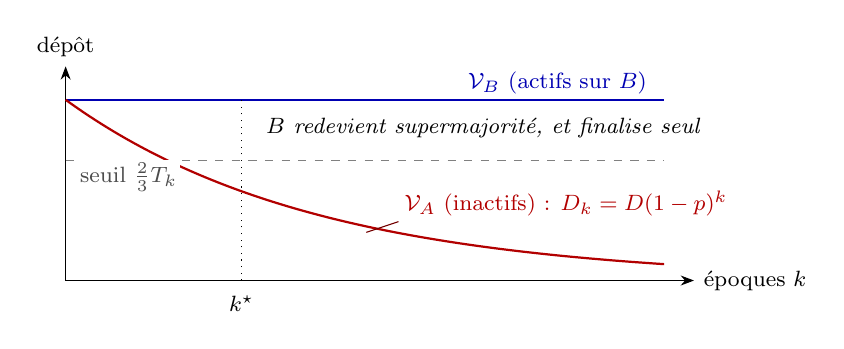
\begin{tikzpicture}[>=Stealth, xscale=0.95, yscale=0.85]
\draw[->] (0,0)--(8.4,0) node[right,font=\footnotesize] {époques $k$};
\draw[->] (0,0)--(0,3.2) node[above,font=\footnotesize] {dépôt};
\draw[thick, blue!70!black] (0,2.7)--(8,2.7);
\node[font=\footnotesize, blue!70!black, anchor=east] at (7.9,2.95) {$\Vv_B$ (actifs sur $B$)};
\draw[thick, red!70!black, domain=0:8, samples=60, smooth]
   plot (\x, {2.7*exp(-0.30*\x)});
\draw[red!45!black, thin] (4.45,0.88)--(4.02,0.72);
\node[font=\footnotesize, red!70!black, anchor=south west] at (4.4,0.82) {$\Vv_A$ (inactifs) : $D_k=D(1-p)^k$};
\draw[dashed, gray] (0,1.8)--(8,1.8);
\node[font=\footnotesize, gray!60!black, anchor=west, fill=white, inner sep=1pt] at (0.15,1.55) {seuil $\tfrac23 T_k$};
\draw[dotted] (2.35,0)--(2.35,2.7);
\node[font=\footnotesize] at (2.35,-0.35) {$k^\star$};
\node[font=\footnotesize, align=left, anchor=west] at (2.55,2.28)
  {\itshape $B$ redevient supermajorité, et finalise seul};
\end{tikzpicture}

{\footnotesize\itshape Figure 3 --- Fuite d'inactivité~: la vivacité est restaurée sur chaque
branche, au prix de la sûreté entre branches.}
\end{center}

Casper échange donc une sûreté \emph{inconditionnelle} contre une sûreté \emph{sous hypothèse
de synchronie faible}, assortie d'une garantie de vivacité — arbitrage classique et
inévitable, qu'éclairent le théorème CAP et le théorème d'impossibilité FLP. Le protocole
prescrit alors une règle purement locale (« retenir le premier point finalisé que l'on a
vu ») et renvoie l'arbitrage entre les deux branches hors du protocole, à une décision
humaine.

%=====================================================================
\section*{Suggestions pour le développement}
%=====================================================================

\noindent\fcolorbox{gray}{gray!5}{\begin{minipage}{0.975\linewidth}\small
\textbf{Attention.} Il s'agit d'un menu à la carte~: vous pouvez choisir d'étudier certains
points, pas tous, pas nécessairement dans l'ordre, et de façon plus ou moins approfondie.
Vous pouvez aussi vous poser d'autres questions que celles indiquées ci-dessous. Il est très
vivement souhaité que vos investigations comportent une partie traitée sur ordinateur et, si
possible, des représentations graphiques de vos résultats.
\end{minipage}}

\medskip
\begin{enumerate}[leftmargin=2em,itemsep=3pt]
\item Implémenter l'arbre des points de contrôle et les primitives associées (hauteurs,
ancêtre, conflit, plus proche ancêtre commun). Comparer expérimentalement le calcul des
hauteurs n\oe ud par n\oe ud et le balayage unique, sur des arbres aléatoires de formes
variées (chemin, arbre binaire complet, arbre de Galton--Watson).

\item Comparer les deux implantations du calcul de $\Jj$ évoquées en §\ref{sec:algo}
(itération du point fixe, parcours de graphe)~: mesurer les temps sur des instances
aléatoires et confronter aux complexités annoncées. Que devient la comparaison si l'on veut
recalculer $\Jj$ après l'ajout d'un seul lien~?

\item Écrire un vérificateur de fautes et le tester~: engendrer aléatoirement des jeux de
votes valides, comparer la détection quadratique de la condition (II) à la version en
$O(m\log m)$, et vérifier que les témoins produits satisfont bien la
définition~\ref{def:comm}.

\item Illustrer le théorème~\ref{th:safety} par une recherche exhaustive~: sur de petits
arbres et de petits jeux de validateurs, énumérer les ensembles de votes finalisant deux
points en conflit, et mesurer la distribution du capital effectivement confisqué. Retrouve-t-on
la borne $T/3$~? Est-elle atteinte~?

\item Simuler un réseau de validateurs (honnêtes, silencieux, byzantins) avec une latence
aléatoire, et mesurer le délai de finalisation en fonction de la proportion de fautifs et de
la latence. Que se passe-t-il au voisinage du seuil $\tfrac13$~?

\item Étudier la fuite d'inactivité~: simuler une partition du réseau, tracer l'évolution des
dépôts sur chaque branche et déterminer l'instant où chacune finalise. Comparer différentes
formules de fuite (linéaire, géométrique, quadratique en la durée de non-finalisation).

\item Traiter le problème du coût minimal d'une attaque~: programmation dynamique
pseudo-polynomiale, comparaison avec une heuristique gloutonne et avec une recherche
exhaustive. Étudier l'écart $\mu-C$ lorsque les dépôts suivent une loi de puissance, comme
c'est le cas en pratique.

\item Formaliser la définition~\ref{def:noyau} comme plus petit point fixe et discuter
l'apport du théorème de Knaster--Tarski~; envisager une spécification du protocole dans un
formalisme vérifiable (automate, logique temporelle) et vérifier la sûreté par exploration
exhaustive sur de petites instances.

\item Discuter la nécessité du seuil~: montrer qu'aucun protocole de consensus ne peut
tolérer un tiers ou plus de participants byzantins dans un réseau asynchrone, et comparer
l'énoncé obtenu au théorème~\ref{th:safety}.

\item Comparer Casper à \textsc{pbft} et à Tendermint~: hypothèses de synchronie, nombre de
messages échangés par décision, nature de la finalité obtenue, et présence ou non d'une
notion d'imputabilité.
\end{enumerate}

%=====================================================================
\section*{Références}
%=====================================================================
\begin{enumerate}[label={[\arabic*]},leftmargin=2.4em,itemsep=1pt,font=\small]
\item[{[1]}] {\small V.~\textsc{Buterin}, V.~\textsc{Griffith}, \emph{Casper the Friendly
Finality Gadget}, arXiv:1710.09437v4, Ethereum Foundation, 2019.}
\item[{[2]}] {\small M.~\textsc{Castro}, B.~\textsc{Liskov}, \emph{Practical Byzantine Fault
Tolerance}, OSDI, 1999.}
\item[{[3]}] {\small J.~\textsc{Kwon}, \emph{Tendermint: Consensus without Mining}, 2014.}
\item[{[4]}] {\small M.~\textsc{Fischer}, N.~\textsc{Lynch}, M.~\textsc{Paterson},
\emph{Impossibility of Distributed Consensus with One Faulty Process}, J.~ACM, 1985.}
\item[{[5]}] {\small S.~\textsc{Nakamoto}, \emph{Bitcoin: A Peer-to-Peer Electronic Cash
System}, 2008.}
\item[{[6]}] {\small M.~\textsc{Garey}, D.~\textsc{Johnson}, \emph{Computers and
Intractability}, Freeman, 1979 (pour \textsc{Somme-de-Sous-Ensemble}).}
\end{enumerate}

\end{document}
